%%%%%%%%%%%%%%%%%%%%%%
%
%   Work related to the verification of the datasets
%
%%%%%%%%%%%%%%%%%%%%%%

\section{Slices of Datacubes}

\section{Power spectra from Theory}

\TODO{Provide some camb and class power spectra here. }

\section{Powerspectra from Simulations}
\begin{figure}
    \centering
    % \includegraphics[width=\linewidth]{main/test.pdf}
    \includeimage[width=\linewidth]{nine_matter_power_spectra}
  \end{figure}

  \begin{figure}
    \centering
    % \includegraphics[width=\linewidth]{main/test.pdf}
    \includeimage[width=\linewidth]{average_matter_power_spectrum}
  \end{figure}

\section{Powerspectra from Datacubes}

\section{Analytical Bispectra}

\begin{equation}
  B^{(3)}(k_1,k_2,k_3) = 2\mathcal{P}(k_1)\mathcal{P}(k_2)F_2(\vec{k}_1, \vec{k}_2) + \mathrm{cyc}
\end{equation}

\begin{equation}
  F_2(\vec{k}_1,\vec{k}_2) = \frac{5}{7} + \frac{x}{2}\left(\frac{k_1}{k_2}+\frac{k_2}{k_1}\right) + \frac{2}{7}x^2,
\end{equation}
where $x = \hat{\vec{k}}_1 \cdot \hat{\vec{k}}_2 = \cos{\theta_{12}}$, where $\theta_{12}$ is the angle spanned by $\vec{k}_1$ and $\vec{k}_2$. We could thus consequently write: $F_2(\vec{k}_1,\vec{k_2}) = F_2(k_1,k_2,\theta_{12})$

Given $k_1$ and $k_2$ and $\theta_{12}$ we have the following relations \TODO{Include figure here}:

\begin{equation}
  \begin{split}
    \alpha &= \pi-\theta_{12}\\
    \beta &= \pi-\theta_{23}\\
    \gamma &= \pi-\theta_{31}
  \end{split}
\end{equation}

From cosine rule:
\begin{equation}
  k_3 = \sqrt{k_1^2 + k_2^2 - 2k_1k_2\cos\alpha}
\end{equation}

From the rule of sines \TODO{explain more?}:
\begin{equation}
  \begin{split}
    \beta &= \arcsin\left(\frac{k_1}{k_3}\sin\alpha\right)\\
    \gamma &= \arcsin\left(\frac{k_2}{k_3}\sin\alpha\right)
  \end{split}
\end{equation}

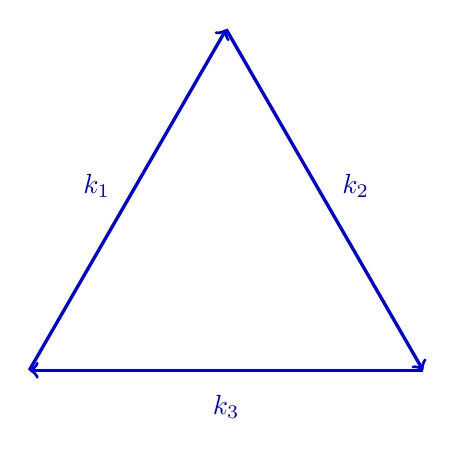
\begin{tikzpicture}
  \colorlet{veccol}{green!70!black}
  \colorlet{vcol}{green!70!black}
  \colorlet{xcol}{blue!85!black}
  \colorlet{projcol}{xcol!60}
  \colorlet{unitcol}{xcol!60!black!85}
  \colorlet{myblue}{blue!70!black}
  \colorlet{myred}{red!90!black}
  \colorlet{mypurple}{blue!50!red!80!black!80}
  \tikzstyle{vector}=[->,very thick,xcol]



  % Define the k vector
  \def\Kone{5}
  \def\Ktwo{5}
  \def\Kthree{5}
  \def\staplelength{1}
  \def\alpha{60}
  \def\beta{60}
  \def\gamma{60}

  \coordinate (k1start) at (0,0);
  \coordinate (k2start) at (\gamma:\Kone);
  \coordinate (k3start) at (\Kthree,0);

  % \Draw vector
  \draw[vector] (k1start) -- (k2start) node[midway, left=20, above=5, right=0] {$\vb{k}_1$};
  \draw[vector] (k2start) -- (k3start) node[midway, right=20, above=5, left=0] {$\vb{k}_2$};
  \draw[vector] (k3start) -- (k1start) node[midway, below=5] {$\vb{k}_3$};
  
  
  % coordinates for the extra stapled lines
  \coordinate (k1staplestop) at ({\Kone*cos(\gamma)+\staplelength*cos(\gamma)}, {\Kone*sin(\gamma)+\staplelength*sin(\gamma)});
  \coordinate (k2staplestop) at ({\Kthree+\staplelength*cos(\beta)}, {-\staplelength*sin(\beta)});
  \coordinate (k3staplestop) at ({-\staplelength*cos(\gamma)}, 0);

  % \draw[dashed] (k2start) -- (k1staplestop);
  % \draw[dashed] (k3start) -- (k2staplestop);
  % \draw[dashed] (k1start) -- (k3staplestop);


  % Template
  % \def\ul{0.52}
  % \def\R{3}
  % \def\ang{60}
  % \coordinate (O) at (0,0);
  % \coordinate (R) at (\ang:\R);
  % \coordinate (X) at ({\R*cos(\ang)},0);
  % \coordinate (Y) at (0,{\R*sin(\ang)});

  % \node[fill=black,circle,inner sep=0.9] (R') at (R) {};
  % \node[above right=-2] at (R') {$(x,y)$};
  % \draw[<->,line width=0.9] %very thick
  %   ({1.2*\R*cos(\ang)},0) -- (O) -- (0,{1.3*\R*sin(\ang)});
  % \draw[projcol,dashed] (X) -- (R);
  % \draw[projcol,dashed] (Y) -- (R);
  % \draw[vector] (O) -- (R') node[midway,left=5,above right=0] {$\vb{r}$};
  % \draw[vector,<->,unitcol]
  %   (\ul,0) node[scale=1,left=2,below left=0] {$\vu{x}$} -- (O) --
  %   (0,\ul) node[scale=1,below=2,below left=0] {$\vu{y}$};
  % \draw pic[->,thick,"$\theta$",draw=black,angle radius=26,angle eccentricity=1.3]
  %   {angle = X--O--R};
  % \draw[thick] (X)++(0,0.1) --++ (0,-0.2) node[scale=0.9,below=-1] {$x = r\cos\theta$};
  % \draw[thick] (Y)++(0.1,0) --++ (-0.2,0) node[scale=0.9,left] {$y = r\sin\theta$};
\end{tikzpicture}

\section{Bispectra from Cube}

